% Introductory slides: Linear Leios and Categorical Crypto.
% Build with LuaLaTeX (the Agda excerpts are Unicode), from this directory:
%   nix build                      # writes result/leios-cc-intro.pdf
% or, to iterate, in `nix develop`:
%   dot -Tpdf -Glabel= -Gbgcolor=transparent ../linear-rules.dot -o linear-rules.pdf
%   lualatex -shell-escape leios-cc-intro.tex
% (-shell-escape lets minted run Pygments for the Agda highlighting.)
\documentclass[aspectratio=169,10pt]{beamer}

\usetheme[numbering=fraction, progressbar=frametitle]{metropolis}

\usepackage{fontspec}
\usepackage{minted}
\usepackage{booktabs}
\usepackage{tikz}
\usetikzlibrary{arrows.meta,positioning,fit,calc,decorations.pathreplacing}

% Agda identifiers use symbols outside DejaVu Sans Mono (ℰ, ⨂, …), so fall
% back to a math font for those glyphs.  This overrides Metropolis's Fira Mono,
% which covers even fewer of them.
\directlua{luaotfload.add_fallback("agdafallback",
  {"NotoSansMath:mode=harf;", "DejaVuSans:mode=harf;"})}
\setmonofont{DejaVu Sans Mono}[Scale=0.8, RawFeature={fallback=agdafallback}]

\definecolor{rb}{RGB}{31,119,180}
\definecolor{eb}{RGB}{255,127,14}
\definecolor{vt}{RGB}{44,160,44}
\definecolor{adv}{RGB}{214,39,40}

% Agda listings sit on a light grey fill, a shade darker than Metropolis's
% background.  `|...|` escapes to LaTeX inside them (for hand-placed colours).
\definecolor{codebg}{gray}{0.93}
\setminted{fontsize=\footnotesize, escapeinside=||,
  bgcolor=codebg, bgcolorpadding=1.5mm}
\newcommand{\agda}[1]{\texttt{#1}}

\tikzset{
  machine/.style={draw, thick, rounded corners=2pt, fill=blue!6,
                  minimum height=8mm, minimum width=18mm, align=center},
  chan/.style={thick, {Latex[length=2mm]}-{Latex[length=2mm]}},
  advchan/.style={chan, adv},
  lbl/.style={font=\scriptsize\ttfamily},
}

\title{Linear Leios in Agda}
\subtitle{An introduction to the protocol and to Categorical Crypto}
\author{Yves Hauser}
\institute{Input Output}
\date{\today}

\begin{document}

\maketitle

\begin{frame}{Outline}
  \tableofcontents
\end{frame}

% ===========================================================================
\section{Linear Leios}
% ===========================================================================

\begin{frame}{Why Linear Leios?}
  \begin{itemize}
    \item Ouroboros Praos: in every slot, each stake pool privately checks
          whether it may produce a block, so a slot can have no leader,
          one, or several.
    \item A block must diffuse before the next one is likely to be
          produced, so throughput is bounded by the block size that
          diffuses in time, not by bandwidth or CPU.
    \item Linear Leios (CIP-0164) lifts that bound:
      \begin{itemize}
        \item \textcolor{rb}{ranking blocks} (RBs) keep the Praos chain and
              its security argument, and each announces at most one EB;
        \item large \textcolor{eb}{endorser blocks} (EBs) carry the
              transactions, diffused off the critical path;
        \item a stake-based committee \textcolor{vt}{votes} on an EB, and a
              \emph{certificate} in the next RB makes it part of the ledger.
      \end{itemize}
  \end{itemize}
\end{frame}

\begin{frame}{Linear Leios in one picture}
  \centering
  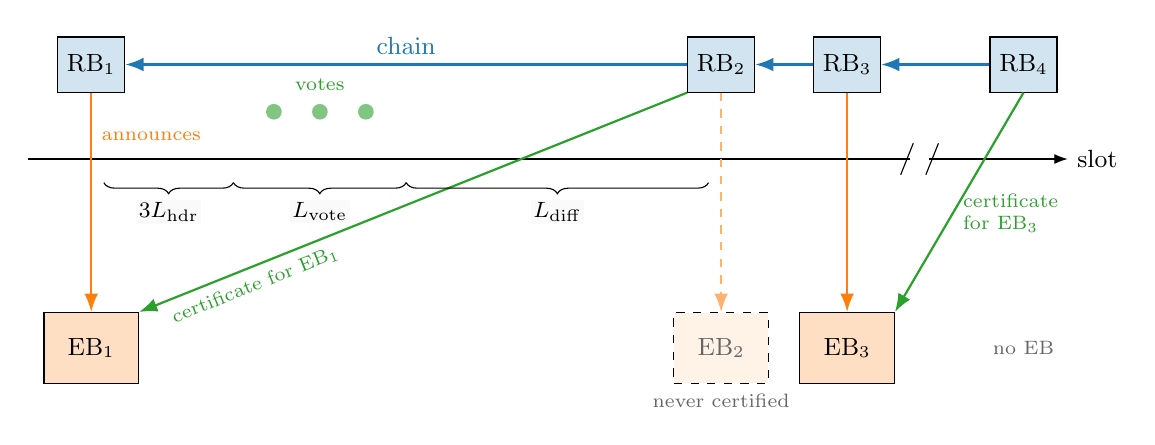
\begin{tikzpicture}[x=0.8cm, y=1cm, every node/.style={font=\small}]
    % slot axis, broken between RB₃ and RB₄: certifying EB₃ needs another
    % 3L_hdr + L_vote + L_diff slots, too wide to draw to scale
    \draw (0,0) -- (14,0);
    \draw (13.85,-0.2) -- (14.05,0.2) (14.25,-0.2) -- (14.45,0.2);
    \draw[-{Latex}] (14.3,0) -- (16.5,0) node[right]{slot};
    % RB chain
    \node[draw, fill=rb!20, minimum size=7mm] (rb1) at (1,1.2) {RB$_1$};
    \node[draw, fill=rb!20, minimum size=7mm] (rb2) at (11,1.2) {RB$_2$};
    \draw[-{Latex}, thick, rb] (rb2) -- node[above]{chain} (rb1);
    \node[draw, fill=rb!20, minimum size=7mm] (rb3) at (13,1.2) {RB$_3$};
    \draw[-{Latex}, thick, rb] (rb3) -- (rb2);
    \node[draw, fill=rb!20, minimum size=7mm] (rb4) at (15.8,1.2) {RB$_4$};
    \draw[-{Latex}, thick, rb] (rb4) -- (rb3);
    % EB
    \node[draw, fill=eb!25, minimum width=12mm, minimum height=9mm] (eb) at (1,-2.4) {EB$_1$};
    \draw[-{Latex}, eb, thick] (rb1) -- node[pos=0.2, right, font=\scriptsize]{announces} (eb);
    % RB₃ follows RB₂ too soon for EB₂ to be certified
    \node[draw, dashed, fill=eb!10, text=black!60, minimum width=12mm, minimum height=9mm]
      (eb2) at (11,-2.4) {EB$_2$};
    \draw[-{Latex}, eb!60, thick, dashed] (rb2) -- (eb2);
    \node[below, font=\scriptsize, text=black!60] at (eb2.south) {never certified};
    % RB₃ announces a fresh EB in turn
    \node[draw, fill=eb!25, minimum width=12mm, minimum height=9mm] (eb3) at (13,-2.4) {EB$_3$};
    \draw[-{Latex}, eb, thick] (rb3) -- (eb3);
    % RB₄ certifies EB₃ and announces nothing
    \draw[-{Latex}, thick, vt] (rb4.south) -- node[right, font=\scriptsize, align=left, pos=0.55]{certificate\\for EB$_3$} (eb3.north east);
    \node[font=\scriptsize, text=black!60] at (15.8,-2.4) {no EB};
    % certificate, drawn first so that the phase labels sit on top of it
    \draw[-{Latex}, thick, vt] (rb2.south west) -- node[pos=0.8, below, sloped, font=\scriptsize]{certificate for EB$_1$} (eb.north east);
    % phases, in the proportions of the CIP's parameters: 3L_hdr : L_vote : L_diff
    % = 3 : 4 : 7 over the 9.6 units from 1.2 to 10.8
    \tikzset{phase/.style={below=6pt, font=\footnotesize, fill=black!2, inner sep=1pt}}
    \draw[decorate, decoration={brace, amplitude=4pt, mirror}]
      (1.2,-0.3) -- node[phase]{$3L_\mathrm{hdr}$} (3.257,-0.3);
    \draw[decorate, decoration={brace, amplitude=4pt, mirror}]
      (3.257,-0.3) -- node[phase]{$L_\mathrm{vote}$} (6,-0.3);
    \draw[decorate, decoration={brace, amplitude=4pt, mirror}]
      (6,-0.3) -- node[phase]{$L_\mathrm{diff}$} (10.8,-0.3);
    % votes, inside the voting window
    \foreach \x in {3.9,4.63,5.36} {
      \node[circle, fill=vt!60, inner sep=2pt] at (\x,0.6) {};
    }
    \node[vt, font=\scriptsize] at (4.63,0.95) {votes};
  \end{tikzpicture}

  \vspace{2mm}
  \small RB$_2$ carries a certificate for EB$_1$ announced by RB$_1$.\\RB$_3$ came too soon after RB$_2$ and EB$_2$ is therefore never certified.\\RB$_3$ announces EB$_3$ in its place, which RB$_4$ certifies without announcing an EB of its own.
\end{frame}

\begin{frame}[fragile]{Blocks and parameters}
  \begin{itemize}
    \item A ranking block announces at most one EB, and carries either
          transactions or a certificate:
  \end{itemize}
\begin{minted}{agda}
mkRB : LeiosState → Maybe EBCert → RankingBlock
mkRB s mc = record
  { announcedEB = proposedEB
  ; txsOrEbCert = maybe inj₂ (inj₁ (proj₁ (splitTxs ToPropose))) mc }
\end{minted}
  \begin{itemize}
    \item A certificate is called for once the announced EB is old enough
          for its votes to have diffused:
  \end{itemize}
\begin{minted}{agda}
certRequest s = find (λ eb → ¿ just (hash eb) ≡ getCurrentEBHash s
                       × slotNumber eb + 3 * Lhdr + Lvote + Ldiff ≤ slot ¿) EBs
\end{minted}
  \begin{itemize}
    \item Votes and certificates are keyed by the hash of the
          \emph{announcing} RB (CIP-0164, ``Vote Structure'').
  \end{itemize}
\end{frame}

\begin{frame}[fragile]{The node as a state machine}
  \begin{itemize}
    \item One relation \agda{\_-⟦\_/\_⟧⇀\_}: state, one input message,
          at most one output message, new state.
  \end{itemize}
\begin{minted}{agda}
data _-⟦_/_⟧⇀_ : MachineType ((FFD ⊗₀ BaseIO) ⊗₀ VotingC) (IO ⊗₀ Adv) LeiosState where
\end{minted}
  \begin{itemize}
    \item Every slot a node must settle four duties before time advances:
  \end{itemize}
\begin{minted}{agda}
data SlotUpkeep : Type where
  Base CertCheck EB-Role VT-Role : SlotUpkeep

allDone s = VT-Role ∈ˡ u × EB-Role ∈ˡ u × Base ∈ˡ u × CertCheck ∈ˡ u
\end{minted}
  \begin{itemize}
    \item A role is settled either by performing it or by
          \emph{provably} declining it (\agda{No-EB-Role},
          \agda{No-VT-Role}).
    \item So an honest node cannot silently skip a block or a vote it
          could have produced.
  \end{itemize}
\end{frame}

\begin{frame}{The transition rules}
  \centering\small
  \begin{tabular}{@{}lll@{}}
    \toprule
    Group & Rules & Effect \\
    \midrule
    Network, ledger & \agda{Slot}, \agda{Chain}, \agda{Fetch}
      & advance the slot, track the base chain \\
    Mempool & \agda{Mempool} & replace the transaction selection \\
    Base chain & \agda{Base₁}, \agda{Base₂}
      & submit an RB, or query for a certificate \\
    Certificates & \agda{Cert₁}, \agda{Cert₂}, \agda{Cert₃}
      & embed, discard, or re-query \\
    Roles & \agda{EB-Role}, \agda{No-EB-Role} & propose an EB, or decline \\
          & \agda{VT-Role}, \agda{No-VT-Role}, \agda{VT-Defer}
      & vote, decline, or postpone \\
    \bottomrule
  \end{tabular}

  \vspace{4mm}
  \begin{itemize}
    \item Premises are decidable; \agda{genPremises} derives the decision
          procedures used by the executable trace verifier.
  \end{itemize}
\end{frame}

% Rendered by the build from ../linear-rules.dot (see flake.nix).
\begin{frame}{The rules over one slot}
  % Wider than the text block: the labels are small at any size.
  \centering
  \makebox[\textwidth]{\includegraphics[width=0.98\paperwidth]{linear-rules.pdf}}
\end{frame}

% One slide per rule of _-⟦_/_⟧⇀_, copied verbatim from
% Leios/Linear.lagda.md.

\begin{frame}[fragile]{Rule \agda{Slot}: advance the slot}
\begin{minted}{agda}
Slot : let open LeiosState s in
      ∙ allDone s
      ──────────────────────────────────────────────────────────────────
      s -⟦ ((ϵ ⊗R) ⊗R) ⊗R ↑ᵢ FFD-OUT msgs / just $ ((L⊗ ϵ) ⊗R) ⊗R ↑ₒ FTCH-LDG ⟧⇀
        let s' = s ↑ L.filter (isValid? s) msgs
        in record s'
             { slot       = suc slot
             ; Upkeep     = []
             ; proposedEB = nothing
             }
\end{minted}
  \begin{itemize}
    \item Fires only once all four duties of the slot are settled
          (\agda{allDone}).
    \item Takes in the valid EBs and headers the network delivered, asks
          for the ledger, and resets the duties for the next slot.
  \end{itemize}
\end{frame}

\begin{frame}[fragile]{Rule \agda{Chain}: track the base chain}
\begin{minted}{agda}
Chain : let open LeiosState s in
      ───────────────────────────────────────────────────────────────────
      s -⟦ ((L⊗ ϵ) ⊗R) ⊗R ↑ᵢ BASE-LDG rbs / nothing ⟧⇀ record s { RBs = rbs }
\end{minted}
  \begin{itemize}
    \item The base chain reports its current blocks; the node records them.
    \item No premises: the tip can change at any moment, including between
          a certificate query and its answer (hence \agda{Cert₂},
          \agda{Cert₃}).
  \end{itemize}
\end{frame}

\begin{frame}[fragile]{Rule \agda{Fetch}: report the ledger}
\begin{minted}{agda}
Fetch : let open LeiosState s in
      ───────────────────────────────────────────────────────────────────────────
      s -⟦ L⊗ (ϵ ⊗R) ᵗ¹ ↑ₒ FetchLdgI / just $ L⊗ (ϵ ⊗R) ᵗ¹ ↑ᵢ FetchLdgO Ledger ⟧⇀ s
\end{minted}
  \begin{itemize}
    \item Answers a request for the node's view of the ledger.
    \item Enabled in every state, and leaves the state unchanged.
  \end{itemize}
\end{frame}

\begin{frame}[fragile]{Rule \agda{Mempool}: replace the transaction selection}
\begin{minted}{agda}
Mempool :
        ───────────────────────────────────────────────────────────────────────────
        s -⟦ L⊗ (ϵ ᵗ¹ ⊗R) ᵗ¹ ↑ᵢ SubmitTxs txs / nothing ⟧⇀ record s { ToPropose = txs }
\end{minted}
  \begin{itemize}
    \item The environment hands the node its current selection of
          transactions, which replaces \agda{ToPropose}.
    \item \agda{EB-Role} takes the EB share of it, and the rules that
          submit an RB take the RB share.
    \item No rule removes the transactions they include, so the
          environment must not offer them again.
  \end{itemize}
\end{frame}

\begin{frame}[fragile]{Rule \agda{Base₁}: submit an RB without a certificate}
\begin{minted}{agda}
Base₁   : let open LeiosState s in
        ∙ needsUpkeep Base
        ∙ needsUpkeep CertCheck
        ∙ hasUpkeep EB-Role
        ∙ certRequest s ≡ nothing
        ───────────────────────────────────────────────────────────────────────────
        s -⟦ ((ϵ ⊗R) ⊗R) ⊗R ↑ᵢ SLOT / just $ ((L⊗ ϵ) ⊗R) ⊗R ↑ₒ SUBMIT (mkRB s nothing) ⟧⇀
          addUpkeep (addUpkeep s CertCheck) Base
\end{minted}
  \begin{itemize}
    \item The chain tip calls for no certificate, so the RB carries
          transactions; this settles both \agda{CertCheck} and \agda{Base}.
    \item \agda{hasUpkeep EB-Role}: the EB role is settled first, so the RB
          announces the EB the node diffuses (\agda{proposedEB}).
    \item The base chain only takes the RB into account if the node is its
          block producer for the slot.
  \end{itemize}
\end{frame}

\begin{frame}[fragile]{Rule \agda{Base₂}: query for a certificate}
\begin{minted}{agda}
Base₂   : let open LeiosState s in
        ∙ needsUpkeep CertCheck
        ∙ hasUpkeep EB-Role
        ∙ certRequest s ≡ just eb
        ───────────────────────────────────────────────────────────────────────────
        s -⟦ ((ϵ ⊗R) ⊗R) ⊗R ↑ᵢ SLOT / just $ (L⊗ ϵ) ⊗R ↑ₒ QUERY (hash currentRB) ⟧⇀
          record (addUpkeep s CertCheck) { PendingQuery = just (hash currentRB) }
\end{minted}
  \begin{itemize}
    \item The tip announces an EB whose voting window closed at least
          $L_\mathrm{diff}$ slots ago, so the node asks the voting
          functionality for a certificate.
    \item The query is keyed by the announcing RB, and recorded in
          \agda{PendingQuery}.
    \item \agda{Base} stays open until the answer arrives.
  \end{itemize}
\end{frame}

\begin{frame}[fragile]{Rule \agda{Cert₁}: embed the certificate}
\begin{minted}{agda}
Cert₁ : let open LeiosState s in
      ∙ needsUpkeep Base
      ∙ CertCheck ∈ˡ Upkeep
      ∙ certRequest s ≡ just eb
      ∙ PendingQuery ≡ just (hash currentRB)
      ∙ Maybe.All (λ c → getEBHash c ≡ hash currentRB) c
      ───────────────────────────────────────────────────────────────────
      s -⟦ (L⊗ ϵ) ⊗R ↑ᵢ CERT c / just $ ((L⊗ ϵ) ⊗R) ⊗R ↑ₒ SUBMIT (mkRB s c) ⟧⇀
        record (addUpkeep s Base) { PendingQuery = nothing }
\end{minted}
  \begin{itemize}
    \item Accepts an answer only while a query is outstanding, and only if
          the query still names the \emph{current} tip.
    \item A positive answer must certify the requested RB; a negative one
          (\agda{c = nothing}) yields an RB without a certificate.
  \end{itemize}
\end{frame}

\begin{frame}[fragile]{Rule \agda{Cert₂}: the tip no longer needs a certificate}
\begin{minted}{agda}
Cert₂ : let open LeiosState s in
      ∙ needsUpkeep Base
      ∙ CertCheck ∈ˡ Upkeep
      ∙ certRequest s ≡ nothing
      ∙ PendingQuery ≡ just r
      ───────────────────────────────────────────────────────────────────
      s -⟦ (L⊗ ϵ) ⊗R ↑ᵢ CERT c / just $ ((L⊗ ϵ) ⊗R) ⊗R ↑ₒ SUBMIT (mkRB s nothing) ⟧⇀
        record (addUpkeep s Base) { PendingQuery = nothing }
\end{minted}
  \begin{itemize}
    \item The tip changed while the query was outstanding, and the new tip
          calls for no certificate at all.
    \item The stale answer is discarded and the RB is submitted without a
          certificate, settling \agda{Base} as \agda{Base₁} would.
  \end{itemize}
\end{frame}

\begin{frame}[fragile]{Rule \agda{Cert₃}: the tip moved, query again}
\begin{minted}{agda}
Cert₃ : let open LeiosState s in
      ∙ needsUpkeep Base
      ∙ CertCheck ∈ˡ Upkeep
      ∙ certRequest s ≡ just eb
      ∙ PendingQuery ≡ just r
      ∙ hash currentRB ≢ r
      ───────────────────────────────────────────────────────────────────
      s -⟦ (L⊗ ϵ) ⊗R ↑ᵢ CERT c / just $ (L⊗ ϵ) ⊗R ↑ₒ QUERY (hash currentRB) ⟧⇀
        record s { PendingQuery = just (hash currentRB) }
\end{minted}
  \begin{itemize}
    \item The new tip calls for a certificate on a \emph{different} RB
          than the one queried.
    \item The stale answer is discarded and a fresh query is issued;
          \agda{Base} stays open until that one is answered.
  \end{itemize}
\end{frame}

\begin{frame}{The certificate path}
  \centering
  \begin{tikzpicture}[node distance=8mm and 16mm, every node/.style={font=\small}]
    \node[machine] (b2) {\agda{Base₂}\\[-1mm]{\scriptsize tip calls for a cert}};
    \node[machine, right=of b2] (wait) {waiting\\[-1mm]{\scriptsize \agda{PendingQuery}}};
    \node[machine, right=of wait, yshift=12mm] (c1) {\agda{Cert₁}\\[-1mm]{\scriptsize submit RB + cert}};
    \node[machine, right=of wait] (c2) {\agda{Cert₂}\\[-1mm]{\scriptsize submit RB, no cert}};
    \node[machine, right=of wait, yshift=-12mm] (c3) {\agda{Cert₃}\\[-1mm]{\scriptsize tip moved: re-query}};
    \draw[-{Latex}, thick] (b2) -- node[above, lbl]{QUERY} (wait);
    \draw[-{Latex}, thick] (wait) -- node[above, sloped, lbl]{CERT c} (c1);
    \draw[-{Latex}, thick] (wait) -- node[above, lbl]{CERT c} (c2);
    \draw[-{Latex}, thick] (wait) -- node[below, sloped, lbl]{CERT c} (c3);
    \draw[-{Latex}, thick] (c3.south) |- ++(0,-6mm) -| node[pos=0.25, below, lbl]{QUERY} (wait.south);
  \end{tikzpicture}

  \vspace{3mm}
  \begin{itemize}\small
    \item The chain tip may change between query and answer, so the answer
          is re-validated against the \emph{current} tip.
    \item Every branch eventually discharges the \agda{Base} duty.
  \end{itemize}
\end{frame}

\begin{frame}[fragile]{Rule \agda{EB-Role}: propose an EB}
\begin{minted}[fontsize=\scriptsize]{agda}
EB-Role : let open LeiosState s in
          ∙ CanProposeEB s π eb
          ∙ needsUpkeep EB-Role
          ──────────────────────────────────────────────────
          s -⟦ ((ϵ ⊗R) ⊗R) ⊗R ↑ᵢ SLOT / just $ ((ϵ ⊗R) ⊗R) ⊗R ↑ₒ FFD-IN (Send (ebHeader eb) nothing) ⟧⇀
            rememberProposal (addUpkeep s EB-Role) eb
\end{minted}
\begin{minted}[fontsize=\scriptsize]{agda}
CanProposeEB : LeiosState → VrfPf → EndorserBlock → Type
CanProposeEB s π eb = let open LeiosState s in
  toProposeEB s π ≡ just eb × canProduceEB slot sk-EB (stake s) π
\end{minted}
  \begin{itemize}
    \item \agda{canProduceEB} holds if and only if the node can make an RB
          in this slot; the EB holds the EB share of \agda{ToPropose}, if
          that share is non-empty.
    \item The EB goes to the network, and \agda{proposedEB} records it for
          the RB to announce.
  \end{itemize}
\end{frame}

\begin{frame}[fragile]{Rule \agda{No-EB-Role}: decline to propose}
\begin{minted}{agda}
No-EB-Role : let open LeiosState s in
             ∙ ¬ (∃₂ λ π eb → CanProposeEB s π eb)
             ∙ needsUpkeep EB-Role
             ──────────────────────────────────────────────────
             s -⟦ ((ϵ ⊗R) ⊗R) ⊗R ↑ᵢ SLOT / nothing ⟧⇀ addUpkeep s EB-Role
\end{minted}
  \begin{itemize}
    \item The role is settled without an EB, but only if \emph{no} choice
          of proof and EB would let the node propose one.
    \item So an honest node cannot silently skip an EB it could have
          produced.
  \end{itemize}
\end{frame}

\begin{frame}[fragile]{Rule \agda{VT-Role}: cast a vote}
\begin{minted}[fontsize=\scriptsize]{agda}
VT-Role : ∀ {ebHash slot'} → let open LeiosState s in
        ∙ CanVote s eb ebHash slot'
        ∙ needsUpkeep VT-Role
        ──────────────────────────────────────────────────
        s -⟦ ((ϵ ⊗R) ⊗R) ⊗R ↑ᵢ SLOT / just $ (L⊗ ϵ) ⊗R ↑ₒ CAST (vote sk-VT (hash currentRB)) ⟧⇀
          rememberVote (addUpkeep s VT-Role) eb
\end{minted}
\begin{minted}[fontsize=\scriptsize]{agda}
CanVote : LeiosState → EndorserBlock → EBRef → ℕ → Type
CanVote s eb ebHash slot' = let open LeiosState s in
    getCurrentEBHash s ≡ just ebHash
  × find (λ (_ , eb') → hash eb' ≟ ebHash) EBs' ≡ just (slot' , eb)
  × hash eb ∉ VotedEBs
  × ¬ isEquivocated s eb
  × isValid s (inj₁ (ebHeader eb))
  × slot' ≤ slotNumber eb + Lhdr
  × slotNumber eb + 3 * Lhdr ≤ slot
  × slot ≤ slotNumber eb + 3 * Lhdr + Lvote
  × isValidityChecked slot eb
  × EndorserBlockOSig.txs eb ≢ []
  × inVotingCommittee params (stake s)
  -- Committee membership is by stake; signing also needs a registered key
  × id ∈ˡ L.map poolID PubKeys
\end{minted}
\end{frame}

\begin{frame}[fragile]{Rule \agda{No-VT-Role}: decline to vote}
\begin{minted}{agda}
No-VT-Role : let open LeiosState s in
             ∙ ¬ (∃[ eb ] ∃[ ebHash ] ∃[ slot' ] CanVote s eb ebHash slot')
             ∙ needsUpkeep VT-Role
             ──────────────────────────────────────────────────
             s -⟦ ((ϵ ⊗R) ⊗R) ⊗R ↑ᵢ SLOT / nothing ⟧⇀ addUpkeep s VT-Role
\end{minted}
  \begin{itemize}
    \item The role is settled without a vote, but only if there is
          \emph{nothing} the node could vote on.
  \end{itemize}
\end{frame}

\begin{frame}[fragile]{Rule \agda{VT-Defer}: postpone a vote}
\begin{minted}{agda}
VT-Defer : let open LeiosState s in
         ∙ slot < voteDeadline s
         ∙ needsUpkeep VT-Role
         ──────────────────────────────────────────────────
         s -⟦ ((ϵ ⊗R) ⊗R) ⊗R ↑ᵢ SLOT / nothing ⟧⇀ addUpkeep s VT-Role
\end{minted}
  \begin{itemize}
    \item A node may abstain while the current EB's voting window is still
          open, even when \agda{VT-Role} could fire.
    \item At the deadline \agda{VT-Defer} no longer applies, and
          \agda{No-VT-Role} does not apply while a vote can still be cast:
          a node that can vote must vote by then.
  \end{itemize}
\end{frame}

% ===========================================================================
\section{Categorical Crypto}
% ===========================================================================

\begin{frame}{Categorical Crypto}
  \begin{itemize}
    \item A framework for universally composable (UC) security, built on
          category theory and mechanised in Agda (\agda{--safe}).
    \item Protocols, functionalities, adversaries and environments are all
          categorical data.
    \item UC emulation and its metatheory (reflexivity, transitivity, dummy
          adversary, composition theorem) are proved once, abstractly.
    \item Then instantiated at a concrete model: \alert{machines} that
          communicate over typed \alert{channels}.
    \item For Leios, the concrete layer matters most: it is the language in
          which the specification is written.
  \end{itemize}
\end{frame}

\begin{frame}[fragile]{Channels}
  \begin{columns}[T]
    \begin{column}{0.55\textwidth}
\begin{minted}{agda}
data Mode : Type where
  Out In : Mode

record Channel : Type₁ where
  constructor _⇿_
  field inType outType : Type

I : Channel
I = ⊥ ⇿ ⊥

_ᵀ : Channel → Channel
A ᵀ = A .outType ⇿ A .inType

_⊗₀_ : Channel → Channel → Channel
A ⊗₀ B = (inType A ⊎ inType B)
       ⇿ (outType A ⊎ outType B)
\end{minted}
    \end{column}
    \begin{column}{0.42\textwidth}
      \begin{itemize}
        \item A channel is a pair of message types, one per direction.
        \item \agda{ᵀ} swaps the directions: the other end's view.
        \item \agda{⊗₀} bundles channels side by side; \agda{I} is its unit.
        \item Messages into a bundle are addressed with a selection DSL:
              \agda{(L⊗ ϵ) ⊗R ↑ᵢ m}.
      \end{itemize}
    \end{column}
  \end{columns}
\end{frame}

% CategoricalCrypto/Channel/Selection.agda, with the implicit binders
% (∀ {m m' A B C} →) left out.
\begin{frame}[fragile]{The selection DSL}
\begin{minted}[fontsize=\scriptsize]{agda}
data _[_]⇒[_]ᵍ_ : Channel → Mode → Mode → Channel → Set₁ where
  ϵ   : A [ m ]⇒[ m ]ᵍ A
  _⊗R : A [ m ]⇒[ m' ]ᵍ B → A [ m ]⇒[ m' ]ᵍ B ⊗₀ C
  L⊗_ : A [ m ]⇒[ m' ]ᵍ B → A [ m ]⇒[ m' ]ᵍ C ⊗₀ B
  _ᵗ¹ : A [ m ]⇒[ m' ]ᵍ B → A [ m ]⇒[ ¬ₘ m' ]ᵍ B ᵀ
  _ᵗ² : A [ m ]⇒[ ¬ₘ m' ]ᵍ B → A [ m ]⇒[ m' ]ᵍ B ᵀ

_↑ᵢ_ : A [ In ]⇒[ m' ]ᵍ B → modeType In A → modeType m' B
_↑ₒ_ : A [ Out ]⇒[ m' ]ᵍ B → modeType Out A → modeType m' B
\end{minted}
  \begin{itemize}\small
    \item A path locates channel \agda{A} inside a bundle \agda{B};
          \agda{↑ᵢ} and \agda{↑ₒ} inject an input or output message of
          \agda{A} along it.
    \item Read it from the inside out: \agda{ϵ} is the message's own
          channel, \agda{\_⊗R} puts it on the left of a \agda{⊗₀},
          \agda{L⊗\_} on the right, and \agda{ᵗ¹}, \agda{ᵗ²} cross a
          \agda{ᵀ}, which flips the direction.
    \item In \agda{VT-Role}, the vote leaves on \agda{VotingC}:
  \end{itemize}
\begin{minted}[fontsize=\scriptsize]{agda}
ϵ         : VotingC [ Out ]⇒[ Out ]ᵍ VotingC
L⊗ ϵ      : VotingC [ Out ]⇒[ Out ]ᵍ (FFD ⊗₀ BaseIO) ⊗₀ VotingC
(L⊗ ϵ) ⊗R : VotingC [ Out ]⇒[ Out ]ᵍ ((FFD ⊗₀ BaseIO) ⊗₀ VotingC) ⊗₀ (IO ⊗₀ Adv) ᵀ
\end{minted}
\end{frame}

\begin{frame}[fragile]{Machines}
\begin{minted}{agda}
machine-type S A = S → inType A → Maybe (outType A) → S → Type

record Machine (A B : Channel) : Type₁ where
  field {State} : Type
        stepRel : machine-type State (A ⊗₀ Bᵀ)
\end{minted}
  \begin{center}
    % stepRel ranges over A ⊗₀ Bᵀ: the machine reads inType A and
    % outType B, and writes outType A and inType B.
    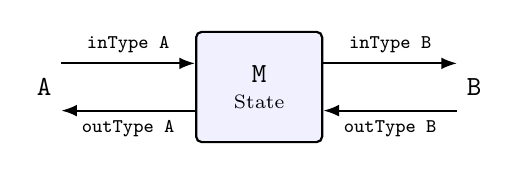
\begin{tikzpicture}[msg/.style={thick, -{Latex[length=2mm]}}]
      \node[machine, minimum width=16mm, minimum height=14mm] (m) {\agda{M}\\[-1mm]{\scriptsize State}};
      \draw[msg] ([xshift=-17mm, yshift=3mm]m.west)
        -- node[above, lbl]{inType A} ([yshift=3mm]m.west);
      \draw[msg] ([yshift=-3mm]m.west)
        -- node[below, lbl]{outType A} ([xshift=-17mm, yshift=-3mm]m.west);
      \draw[msg] ([yshift=3mm]m.east)
        -- node[above, lbl]{inType B} ([xshift=17mm, yshift=3mm]m.east);
      \draw[msg] ([xshift=17mm, yshift=-3mm]m.east)
        -- node[below, lbl]{outType B} ([yshift=-3mm]m.east);
      \node[left] at ([xshift=-17mm]m.west) {\agda{A}};
      \node[right] at ([xshift=17mm]m.east) {\agda{B}};
    \end{tikzpicture}
  \end{center}
  \begin{itemize}
    \item A machine from \agda{A} to \agda{B}: a relation that consumes one
          message and emits at most one.
    \item Relational, so nondeterminism is free: the spec says what an
          honest node \emph{may} do.
    \item Linear Leios is exactly such a relation:
          \agda{LinearLeios .stepRel = \_-⟦\_/\_⟧⇀\_}.
  \end{itemize}
\end{frame}

\begin{frame}[fragile]{Composing machines}
  \begin{columns}[T]
    \begin{column}{0.48\textwidth}
      \centering
      \textbf{Parallel}\\ \agda{M₁ ⊗₁ M₂ : Machine (A ⊗₀ C) (B ⊗₀ D)}

      \vspace{2mm}
      \begin{tikzpicture}
        \node[machine] (m1) {\agda{M₁}};
        \node[machine, below=4mm of m1] (m2) {\agda{M₂}};
        \draw[chan] (m1.west) -- ++(-6mm,0) node[left, lbl]{A};
        \draw[chan] (m1.east) -- ++(6mm,0) node[right, lbl]{B};
        \draw[chan] (m2.west) -- ++(-6mm,0) node[left, lbl]{C};
        \draw[chan] (m2.east) -- ++(6mm,0) node[right, lbl]{D};
        \node[draw, dashed, fit=(m1)(m2), inner sep=2mm] {};
      \end{tikzpicture}

      \vspace{1mm}
      \small State is the product; each step is a step of one component.
    \end{column}
    \begin{column}{0.48\textwidth}
      \centering
      \textbf{Sequential}\\ \agda{M₁ ∘ M₂ : Machine A C}

      \vspace{2mm}
      \begin{tikzpicture}
        % M₂ : Machine A B and M₁ : Machine B C; domain on the left, as on
        % the Machines slide.
        \node[machine, minimum width=12mm] (m2) {\agda{M₂}};
        \node[machine, minimum width=12mm, right=14mm of m2] (m1) {\agda{M₁}};
        \draw[chan] (m2.west) -- ++(-5mm,0) node[left, lbl]{A};
        \draw[chan] (m2) -- node[above, lbl]{B} node[below, lbl]{(hidden)} (m1);
        \draw[chan] (m1.east) -- ++(5mm,0) node[right, lbl]{C};
        \node[draw, dashed, fit=(m1)(m2), inner sep=2mm] {};
      \end{tikzpicture}

      \vspace{1mm}
      \small Messages on \agda{B} bounce internally (\agda{TraceRel}) until
      one leaves on \agda{A} or \agda{C}.
    \end{column}
  \end{columns}
\end{frame}

\begin{frame}[fragile]{Adversaries: composition that keeps side channels}
\begin{minted}{agda}
_∘ᴷ_ : Machine B (C ⊗₀ E₂) → Machine A (B ⊗₀ E₁)
     → Machine A (C ⊗₀ (E₁ ⊗₀ E₂))

_⊗ᴷ_ : Machine A₁ (B₁ ⊗₀ E₁) → Machine A₂ (B₂ ⊗₀ E₂)
     → Machine (A₁ ⊗₀ A₂) ((B₁ ⊗₀ B₂) ⊗₀ (E₁ ⊗₀ E₂))
\end{minted}
  \begin{itemize}
    \item A machine exposes, besides its main interface, an
          \textcolor{adv}{adversary interface} \agda{E}.
    \item \agda{∘ᴷ} and \agda{⊗ᴷ} compose machines and \emph{collect} the
          adversary interfaces instead of hiding them.
    \item Abstractly: a graded Kleisli category, graded by the monoidal
          category of adversary interfaces.
  \end{itemize}
\end{frame}

\begin{frame}[fragile]{When are two machines the same?}
\begin{minted}{agda}
record _≅ᴹ_ (M M' : Machine A B) : Type where
  field to      : S → S'               from    : S' → S
        from∘to : ∀ s  → from (to s) ≡ s    to∘from : ∀ s' → to (from s') ≡ s'
        step-to   : R  s₁  i o s₂  → R' (to s₁)    i o (to s₂)
        step-from : R' s₁' i o s₂' → R  (from s₁') i o (from s₂')
\end{minted}
  \begin{itemize}
    \item \agda{≅ᴹ}: a state bijection that preserves and reflects steps.
    \item Up to \agda{≅ᴹ}, machines with \agda{∘}, \agda{⊗₁}, \agda{I} form
          a \alert{symmetric monoidal category}, all laws proved.
    \item Strong, and sometimes too strong: a bisimulation \agda{\_≈ᴮ\_}
          is available where state spaces differ.
  \end{itemize}
\end{frame}

\begin{frame}{UC emulation}
  \begin{itemize}
    \item Environments are tests: machines into a fixed output channel
          \agda{ℰ-Out}, possibly with an ancilla wire.
    \item \agda{f ≈ℰ g}: every test yields equivalent composites, i.e.\ no
          environment distinguishes \agda{f} from \agda{g}.
    \item \agda{π ≤UC φ}: for every adversary against the real protocol
          \agda{π} there is a simulator against the ideal functionality
          \agda{φ} such that the two worlds are \agda{≈ℰ}.
    \item The abstract layer proves, once, the following:
      \begin{itemize}
        \item \agda{≤UC} is a preorder;
        \item the dummy adversary is complete;
        \item \alert{composition}: if \agda{π ≤UC φ} then
              \agda{ρ ∘ π ≤UC ρ ∘ φ}.
      \end{itemize}
    \item Practical consequence: reason about Leios against an
          \emph{ideal} voting functionality, then replace it.
  \end{itemize}
\end{frame}

% ===========================================================================
\section{Linear Leios as machines}
% ===========================================================================

\begin{frame}[fragile]{The node's interface}
  \begin{columns}[T]
    \begin{column}{0.5\textwidth}
\begin{minted}{agda}
LinearLeios :
  Machine ((FFD ⊗₀ BaseIO) ⊗₀ VotingC)
          (IO ⊗₀ Adv)

data VotingT : Mode → Type where
  CAST  : Vote → VotingT Out
  QUERY : EBRef → VotingT Out
  CERT  : Maybe EBCert → VotingT In
\end{minted}
    \end{column}
    \begin{column}{0.46\textwidth}
      \centering
      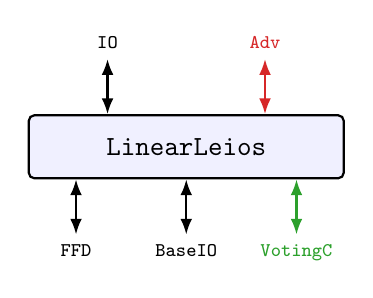
\begin{tikzpicture}
        \node[machine, minimum width=40mm] (ll) {\agda{LinearLeios}};
        \draw[chan] ([xshift=-10mm]ll.north) -- ++(0,7mm) node[above, lbl]{IO};
        \draw[advchan] ([xshift=10mm]ll.north) -- ++(0,7mm) node[above, lbl]{Adv};
        \draw[chan] ([xshift=-14mm]ll.south) -- ++(0,-7mm) node[below, lbl]{FFD};
        \draw[chan] (ll.south) -- ++(0,-7mm) node[below, lbl]{BaseIO};
        \draw[chan, vt] ([xshift=14mm]ll.south) -- ++(0,-7mm) node[below, lbl]{VotingC};
      \end{tikzpicture}
    \end{column}
  \end{columns}
  \begin{itemize}
    \item \agda{FFD}: freshest-first diffusion of EB headers and bodies.
    \item \agda{BaseIO}: the base chain (Praos) as an abstract functionality.
    \item \agda{VotingC}: casting votes and querying for certificates.
    \item \agda{IO}: slots, transactions, ledger queries from the
          environment.
  \end{itemize}
\end{frame}

\begin{frame}{One honest node: \texttt{Leios1 = ext-spec ∘ᴷ spec}}
  \centering
  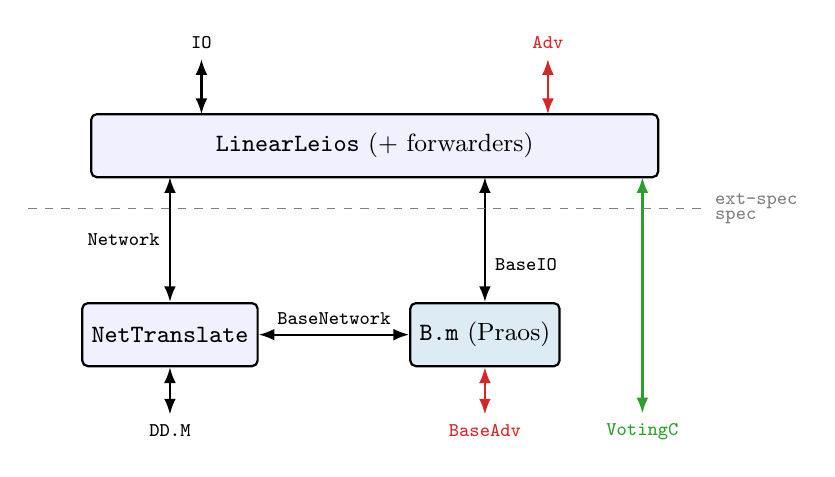
\begin{tikzpicture}[x=1mm, y=1mm, every node/.style={font=\small}]
    \node[machine, minimum width=72mm] (ll) at (0,0) {\agda{LinearLeios} (+ forwarders)};
    \node[machine] (nt) at (-26,-24) {\agda{NetTranslate}};
    \node[machine, fill=rb!15] (bm) at (14,-24) {\agda{B.m} (Praos)};
    \draw[chan] (-22,4) -- ++(0,7) node[above, lbl]{IO};
    \draw[advchan] (22,4) -- ++(0,7) node[above, lbl]{Adv};
    \draw[chan] (-26,-4) -- node[left, lbl]{Network} (nt.north);
    \draw[chan] (14,-4) -- node[pos=0.7, right, lbl]{BaseIO} (bm.north);
    \draw[chan] (bm.west) -- node[above, lbl]{BaseNetwork} (nt.east);
    \draw[advchan] (bm.south) -- ++(0,-6) node[below, lbl]{BaseAdv};
    \draw[chan] (nt.south) -- ++(0,-6) node[below, lbl]{DD.M};
    \draw[chan, vt] (34,-4) -- ++(0,-30) node[below, lbl]{VotingC};
    \draw[dashed, gray] (-44,-8) -- (42,-8) node[right, lbl, gray, align=left]{ext-spec\\[-1mm]spec};
  \end{tikzpicture}

  \vspace{2mm}
  \begin{itemize}\small
    \item \agda{spec}: the Praos node \agda{B.m} with Leios' messages
          multiplexed onto the same diffusion network.
    \item \agda{ext-spec}: the Leios layer on top; its adversary interface
          is collected by \agda{∘ᴷ}.
  \end{itemize}
\end{frame}

\begin{frame}[fragile]{A deployment}
\begin{minted}{agda}
network = liftᴷ (shuffle numberOfParties DD.M VotingC)
            ∘ᴷ (DD.Network ⊗ᴷ Certifier.Functionality) ∘ idᴷ
\end{minted}
  \begin{itemize}
    \item $n$ parties; honest ones run \agda{Leios1}, the others arbitrary
          machines with the same channels.
    \item Shared functionalities: a delayed-diffusion network
          (delay \agda{k}) and a \agda{Certifier} for votes.
    \item \agda{shuffle} regroups $n$ network ports and $n$ voting ports into
          one \agda{DD.M ⊗₀ VotingC} port per party.
    \item Voting is a channel, so the certifier can be swapped:
      \begin{itemize}
        \item \agda{Voting.Ideal}: certificate correctness is proved;
        \item \agda{Voting.Voter}: a local, real voter that answers queries
              from its own vote log.
      \end{itemize}
  \end{itemize}
\end{frame}

% ===========================================================================
\section{Linear Leios properties}
% ===========================================================================

\begin{frame}[fragile]{Safety: common prefix}
\begin{minted}{agda}
safeState : {A : Channel} → ℕ → (E : Environment A) → Machine.State (protocol E) → Type
safeState k E S =
  {p p' : Fin n} (honest-p : p ∈ honest-nodes) (honest-p' : p' ∈ honest-nodes)
  → prune k (getChain E S honest-p) ≼ getChain E S honest-p'

safety : ℕ → Type₁
safety k = ∀ {A} (E : Environment A) → Invariant (protocol E) (safeState k E)

Invariant : (P : State → Type) → Type
Invariant P = (s₁ s₂ : State) → Trace s₁ s₂ → P s₁ → P s₂
\end{minted}
  \begin{itemize}
    \item Cutting the last \agda{k} blocks off one honest chain leaves a
          prefix of any other.
    \item \agda{protocol E = E ∘ (nodes ∘ᴷ network)}: the deployment,
          closed off by an environment that also plays the adversary.
    \item An invariant over every environment: traces preserve safe states.
    \item \agda{getChain} reads a chain through the node's
          \agda{IsBlockchain} queries.
  \end{itemize}
\end{frame}

\begin{frame}[fragile]{Liveness: chain growth and chain quality}
\begin{minted}{agda}
hcgState : {A : Channel} → ℚ → (E : Environment A) → Machine.State (protocol E) → Type
hcgState τ E S₀ =
    {p : Fin n} (hp : p ∈ honest-nodes) {pref suff : List Block} {b : Block}
  → getChain E S₀ hp ≡ pref ++ (b ∷ suff)
  → isHonestBlock b
  → τ ℚ.* ℕ→ℚ (getSlot E S₀ hp ∸ slotOf b) ℚ.≤ ℕ→ℚ (length suff)

∃cqState : {A : Channel} → ℕ → (E : Environment A) → Machine.State (protocol E) → Type
∃cqState T E S₀ =
    {p : Fin n} (hp : p ∈ honest-nodes)
  → Any.Any isHonestBlock (recent T (getSlot E S₀ hp) (getChain E S₀ hp))
\end{minted}
  \begin{itemize}
    \item \textbf{Honest chain growth}: at least
          $\tau \cdot (\mathit{slot} - \mathit{slot}_b)$ blocks follow an
          honest block \agda{b}.
    \item \textbf{Existential chain quality}: among the blocks of the last
          \agda{T} slots of an honest chain, at least one is honest.
    \item \agda{hcg τ} and \agda{∃cq T} are invariants over every
          environment, like \agda{safety k}.
  \end{itemize}
\end{frame}

\begin{frame}[fragile]{What is proved}
  \begin{itemize}
    \item \textbf{Certificate correctness} (ideal voting): if a
          certificate for a block exists, an honest node validated it,
          provided the adversary holds fewer than \agda{threshold} seats.
    \item \textbf{Safety transfer}: Leios inherits common prefix from the
          base chain.
  \end{itemize}
\begin{minted}{agda}
leiosSafety : (∀ {A} (E : S.Environment A) → TrM.ChainLemma-ty E)
            → Deployment.safety Tr.base k → S.safety k
\end{minted}
  \begin{itemize}
    \item \textbf{Liveness transfer}: honest chain growth and chain quality
          (\agda{leiosHCG}, \agda{leios∃CQ}), from chain and slot lemmas.
    \item The key step is \agda{is-extension}: the Leios node \emph{is}
          the base node with an extra layer on top, up to \agda{≅ᴹ}.
  \end{itemize}
\end{frame}

\begin{frame}{Status and open questions}
  \begin{itemize}
    \item Discharge the chain and slot lemmas for all environments, so the
          transfer theorems become unconditional.
    \item A progress theorem: enough traces exist, so invariants are not
          vacuous.
    \item Real voting \agda{≤UC} ideal voting:
      \begin{itemize}
        \item needs synchrony between diffusion delay \agda{k} and
              $L_\mathrm{diff}$;
        \item needs a simulation relation weaker than \agda{≅ᴹ}.
      \end{itemize}
    \item Instantiating the base chain with the Praos specification.
    \item Conformance: the executable trace verifier checks simulator
          traces against these rules.
  \end{itemize}
\end{frame}

\begin{frame}{Summary}
  \begin{itemize}
    \item Linear Leios: one EB per RB, committee votes, certificate in a
          later RB.
    \item Specified as a relational state machine with per-slot duties.
    \item Categorical Crypto gives typed channels, machines, composition
          with adversary interfaces, and an abstract UC theory.
    \item The node, the network and voting are separate machines, wired by
          \agda{∘}, \agda{⊗₁}, \agda{∘ᴷ}, \agda{⊗ᴷ}.
    \item Security of Leios is \emph{transferred} from the base chain rather
          than proved from scratch.
  \end{itemize}
  \vfill
  \centering\small
  \url{https://github.com/input-output-hk/ouroboros-leios-formal-spec}\\
  \url{https://github.com/input-output-hk/categorical-crypto}
\end{frame}

\end{document}
